\documentclass[12pt]{article}

\usepackage{cite}
\usepackage{amsmath,amsfonts,amssymb}
\usepackage{multirow}
\usepackage{graphicx}
\usepackage{float} % Allows putting an [H] in \begin{figure} to specify the exact location of the figure
\graphicspath{{./Plots/}} % Specifies the directory where pictures are stored

\usepackage{hyperref}

\usepackage{listings} % Required for inserting code snippets
\usepackage[usenames,dvipsnames]{color} % Required for specifying custom colors and referring to colors by name

\definecolor{DarkGreen}{rgb}{0.0,0.4,0.0} % Comment color
\definecolor{highlight}{RGB}{255,251,204} % Code highlight color

\lstdefinestyle{Style1}{ % Define a style for your code snippet, multiple definitions can be made if, for example, you wish to insert multiple code snippets using different programming languages into one document
language=R, % Detects keywords, comments, strings, functions, etc for the language specified
backgroundcolor=\color{highlight}, % Set the background color for the snippet - useful for highlighting
basicstyle=\footnotesize\ttfamily, % The default font size and style of the code
breakatwhitespace=false, % If true, only allows line breaks at white space
breaklines=true, % Automatic line breaking (prevents code from protruding outside the box)
captionpos=b, % Sets the caption position: b for bottom; t for top
commentstyle=\usefont{T1}{pcr}{m}{sl}\color{DarkGreen}, % Style of comments within the code - dark green courier font
deletekeywords={}, % If you want to delete any keywords from the current language separate them by commas
%escapeinside={\%}, % This allows you to escape to LaTeX using the character in the bracket
firstnumber=1, % Line numbers begin at line 1
frame=single, % Frame around the code box, value can be: none, leftline, topline, bottomline, lines, single, shadowbox
frameround=tttt, % Rounds the corners of the frame for the top left, top right, bottom left and bottom right positions
%keywordstyle=\color{Blue}\bf, % Functions are bold and blue
morekeywords={}, % Add any functions no included by default here separated by commas
numbers=left, % Location of line numbers, can take the values of: none, left, right
numbersep=10pt, % Distance of line numbers from the code box
numberstyle=\tiny\color{Gray}, % Style used for line numbers
rulecolor=\color{black}, % Frame border color
showstringspaces=false, % Don't put marks in string spaces
showtabs=false, % Display tabs in the code as lines
stepnumber=5, % The step distance between line numbers, i.e. how often will lines be numbered
stringstyle=\color{Purple}, % Strings are purple
tabsize=2, % Number of spaces per tab in the code
}

\lstdefinestyle{Style2}{ % Define a style for your code snippet, multiple definitions can be made if, for example, you wish to insert multiple code snippets using different programming languages into one document
language=Perl, % Detects keywords, comments, strings, functions, etc for the language specified
backgroundcolor=\color{highlight}, % Set the background color for the snippet - useful for highlighting
basicstyle=\footnotesize\ttfamily, % The default font size and style of the code
breakatwhitespace=false, % If true, only allows line breaks at white space
breaklines=true, % Automatic line breaking (prevents code from protruding outside the box)
captionpos=b, % Sets the caption position: b for bottom; t for top
commentstyle=\usefont{T1}{pcr}{m}{sl}\color{DarkGreen}, % Style of comments within the code - dark green courier font
deletekeywords={}, % If you want to delete any keywords from the current language separate them by commas
%escapeinside={\%}, % This allows you to escape to LaTeX using the character in the bracket
firstnumber=1, % Line numbers begin at line 1
frame=single, % Frame around the code box, value can be: none, leftline, topline, bottomline, lines, single, shadowbox
frameround=tttt, % Rounds the corners of the frame for the top left, top right, bottom left and bottom right positions
%keywordstyle=\color{Blue}\bf, % Functions are bold and blue
morekeywords={}, % Add any functions no included by default here separated by commas
numbers=left, % Location of line numbers, can take the values of: none, left, right
numbersep=10pt, % Distance of line numbers from the code box
numberstyle=\tiny\color{Gray}, % Style used for line numbers
rulecolor=\color{black}, % Frame border color
showstringspaces=false, % Don't put marks in string spaces
showtabs=false, % Display tabs in the code as lines
stepnumber=5, % The step distance between line numbers, i.e. how often will lines be numbered
stringstyle=\color{Purple}, % Strings are purple
tabsize=2, % Number of spaces per tab in the code
}

% Create a command to cleanly insert a snippet with the style above anywhere in the document
\newcommand{\insertcode}[2]{\begin{itemize}\item[]\lstinputlisting[caption=#2,label=#1,style=Style1]{#1}\end{itemize}} % The first argument is the script location/filename and the second is a caption for the listing

\newcommand{\insertresult}[2]{\begin{itemize}\item[]\lstinputlisting[caption=#2,label=#1,style=Style2]{#1}\end{itemize}}


\newtheorem{theorem}{Theorem}
\newtheorem{lemma}{Lemma}
\newtheorem{corollary}{Corollary}
\newtheorem{proposition}{Proposition}
\newtheorem{algorithm}{Algorithm}
\newtheorem{remark}{Remark}
\newtheorem{example}{Example}
\newtheorem{condition}{Condition}

\begin{document}

\section{Introduction}

\subsection{What is the YPmodel package?}
The YPmodel package is an add-on package for the R \cite{team2008r} statistical computing system. It provides functions for the analysis of the comparison of failure times between a treated and control group under independent censorship, based on several research works by Song et al \cite{yang2005semiparametric,yang2009improved,yang2011estimation,yang2012checking}.
All comments, criticisms and queries on the package or associated documentation are gratefully
received. Citation information is available at \href{http://cran.r-project.org/web/packages/YPmodel/citation.html}{http://cran.r-project.org/web/packages/YPmodel/citation.html}.

\subsection{Obtaining the package/guide}
The package can be downloaded from CRAN (The Comprehensive R Archive Network) at \href{http:
//cran.r-project.org/}{http:
//cran.r-project.org/}. This guide (in pdf) will be in the directory \textit{YPmodel/doc/}
underneath wherever the package is installed. You can get it by invoking
\insertcode{"Scripts/code0.pl"}{YPmodel help documentation.}
To have a quick overview of what the package does, you might want to have a look at its
own web page \href{http://cran.r-project.org/web/packages/YPmodel/}{http://cran.r-project.org/web/packages/YPmodel/}.

\subsection{Contents}
To help users to use properly the YPmodel packages, this report introduces all main functions in details. Some practical examples are inserted within the text to show how it works in practice. Section \ref{Section.Model} introduces the data format on which the package is based.
Section \ref{Section:estimation} describes how to estimate the model parameters. Section \ref{Section.Intervals} presents functions to estimate confidence intervals and bands for the hazard ratio function. In section  \ref{Section.logrank} and section \ref{Section.LacTest}, we show how to perform several hypothesis tests. Section \ref{Section.All} provides an all-in-one method corresponding to functions through this package. Section \ref{Section.Conclusions} concludes this manual. Note that algorithmic parameters are summarized in the Annex part.

\subsection{Legalese}
This program is free software; you can redistribute it and/or modify it under the terms of the
GNU General Public License as published by the Free Software Foundation; either version 3 of
the License, or (at your option) any later version.
This program is distributed in the hope that it will be useful, but without any warranty;
without even the implied warranty of merchantability or fitness for a particular purpose. See
the GNU General Public License for more details.
A copy of the GNU General Public License can be obtained from \href{http://www.gnu.org/copyleft/gpl.html}{http://www.gnu.org/copyleft/gpl.html}.
%
%\subsection{Acknowledgements}
%...

\section{Preparing Data}\label{Section.Model}
Consider the comparison of failure times between a treated and control group under independent censorship.
Let $T_1, \ldots , T_n$ be the pooled lifetimes of the 2 groups, with $T_1, \ldots , T_{n_1}$, $n_1 < n$, constituting the control group having the survivor function $S_C$.
Let $C_1, \ldots , C_n$ be the censoring variables, and $Z_i = I (i > n_1)$, $i = 1, \ldots, n$, where $I (\cdot)$ is the indicator function.
The available data consist of the independent triplets $(X_i , \delta_i , Z_i )$, $i = 1, \ldots, n$, where $X_i = \min(T_i, C_i)$ and $\delta_i = I (T_i \leq C_i)$.

\subsection{Loading gastric example}\label{gastric.data}
The Gastrointestinal Tumor Study Group (1982) \cite{schein2006comparison} compared chemotherapy with combined chemotherapy and radiation therapy, in the treatment
of locally unresectable gastric cancer. Each treatment arm had $45$ patients, with two observations
of the chemotherapy group and six of the combination group censored. Kaplan-Meier plots of the
two estimated survival curves cross at around $1000$ days.

The study results are included in this package, named as 'gastric'. Before we call this sample data, we first must load the YPmodel (make sure the YPmodel has been installed in R). This can be done as follows:
\insertcode{"Scripts/code3.pl"}{Loading YPmodel package.}
Then we can load the sample data 'gastric' as follows:
\insertcode{"Scripts/code4.pl"}{Loading sample data.}
\insertcode{"Scripts/result4.pl"}{Results of scripts.}
where variables of each column present lifetime vector, censor indicator vector, and group indicator vector, respectively.

\subsection{Inputting Data}
In most cases, we want to use this package to run with our own data sets. In the following example, we demonstrate how to input data in R that can be directly executed by our package.
Assume we have a simple test on one medicine effect, and only six persons were included.
They were divided into treated and control group, where variable $Z$ is the group indicators.
This study lasted for $3$ years, and researchers recorded their observed lifetime (unite: year, variable $X$) and wether or not they quitted or lived over the study's period (variable $\delta$).
Table \ref{Tab:CollectedData} gives the data sample collected:
\begin{table}[!h]
\renewcommand{\arraystretch}{1.3}
\caption{Collected Data} \label{Tab:CollectedData} \centering
\begin{tabular}{|c||c|c|c|}
  \hline
  No & $X$ & $\delta$ & $Z$ \\
  \hline
  1 & 0.0027 & 1 & 0 \\
  2 & 0.8412 & 0 & 0 \\
  3 & 1.3741 & 0 & 1 \\
  4 & 1.8322 & 1 & 0 \\
  5 & 2.471 & 1 & 1 \\
  6 & 3 & 0 & 1 \\
  \hline
\end{tabular}
\end{table}

Before using algorithms in YPmodel, we first need to input this table into an R-based matrix. Let us assume that we want to name the matrix as 'data'. This can be done as follows:
\insertcode{"Scripts/code1.pl"}{Inputting data.}
\insertcode{"Scripts/result1.pl"}{Results of scripts.}
At the end of processing this call, the data matrix will be created.

\begin{remark}
If we recorded the data into a text file (e.g. 'SampleData.txt') with three columns representing $X$, $\delta$ and $Z$ respectively, then we can directly load the table into R-based matrix as follows:
\insertcode{"Scripts/code2.pl"}{Loading data from text files.}
In the YPmodel package, the name of those text files could be used as the input data name. See section \ref{Section.All} for more details.
\end{remark}

\section{Parameter Estimation}\label{Section:estimation}
 The model of Yang and Prentice (YPmodel) will be determined by the parameter $\beta = (\beta_1, \beta_2)^T$ and the baseline function $R(t)$, and \cite{yang2005semiparametric} presented a estimator for them.

To perform the estimator, we will use the function "YPmodel.estimate".
\insertcode{"Scripts/code7 - 2.pl"}{Performing estimator.}
where the dataframe $Estimate$ contains the results of estimator, and Table \ref{Tab:EstimateStructure} gives its structures.

\begin{table}[!h]
\renewcommand{\arraystretch}{1.3}
\caption{Dataframe $Estimate$ Structure} \label{Tab:EstimateStructure} \centering
\begin{tabular}{|c||c|}
  \hline
  Variables & Notes  \\
  \hline
  $beta$ & Value of $\hat{\beta}$. \\
  $r$ & Value of $\hat{R}(t,\hat{\beta})$. \\
  \hline
\end{tabular}
\end{table}

If we want to obtain the value of estimates, then we could use the codes
\insertcode{"Scripts/result13.pl"}{Getting value of $\hat{\beta}$.}

\subsection{Analyzing results for the hazard ratio function}
There are a few summary functions available in the package, including estimators.
To get summary information about the $S3$ object, we can use

\insertcode{"Scripts/code10.pl"}{Summarizing estimates' results.}
or simply,
\insertcode{"Scripts/code10s.pl"}{Summarizing estimates' results.}
\insertcode{"Scripts/result10.pl"}{Summarizing estimates' results.}

We can see that $\hat{\beta}=(1.6,-0.906)^T$ and $\hat{\theta}=(4.9541,0.4041)^T$.
Another summary function is available for plotting the survival functions. This can be done as follows:
\insertcode{"Scripts/code12.pl"}{}
or simply,
\insertcode{"Scripts/code12s.pl"}{Plotting estimates' results.}

\begin{figure}[H]
\center{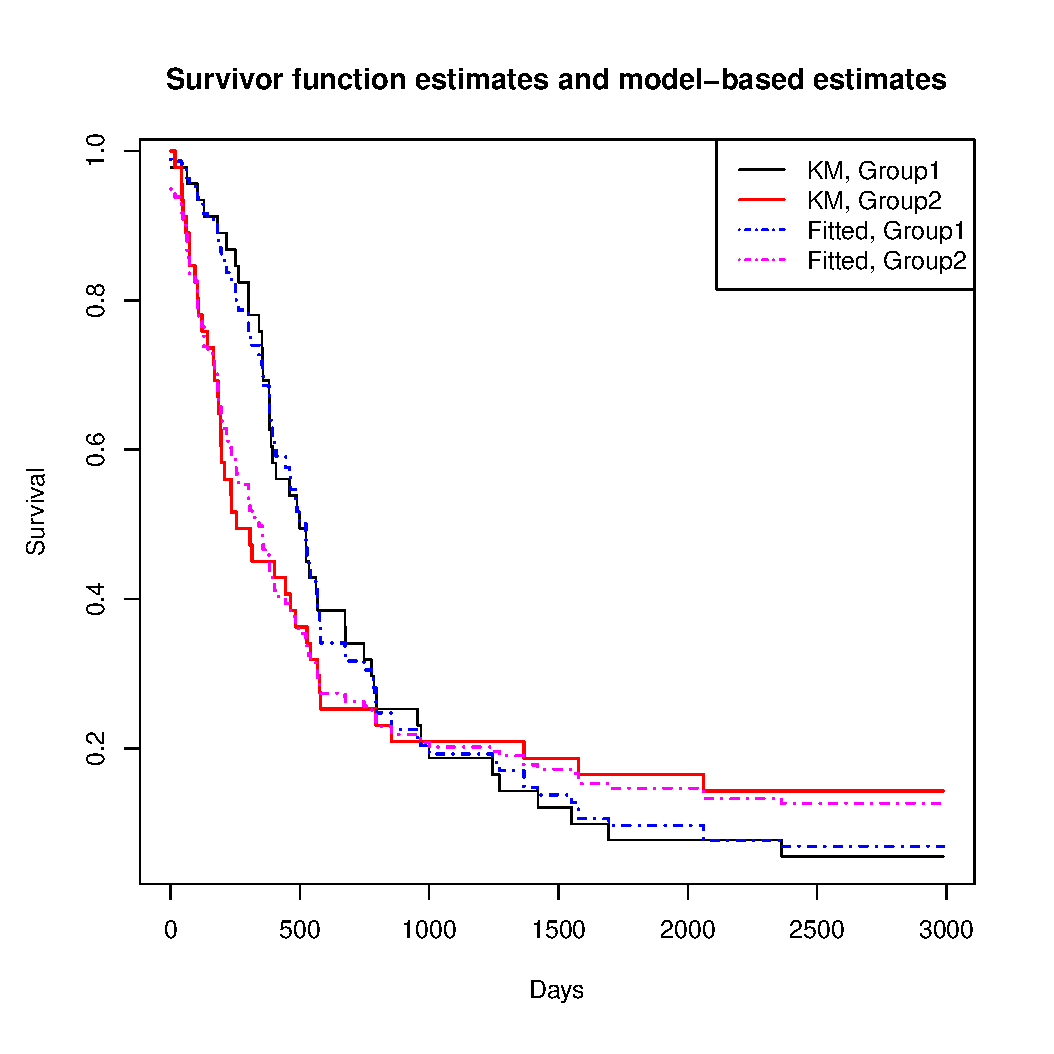
\includegraphics[width=1.0\linewidth]{plot1}}
\caption{Plotting results.}
\label{fig:plot1}
\end{figure}

\subsection{Options}\label{estimiating.confidentialbeta}
In the estimating process, the parameter
\begin{itemize}
  \item $startPoint$ controls the start point of the iteration for $\hat{\beta}$, and the default value is $(0,0)$.
  \item $nm$ controls a bound for $\hat{\beta}$, and the default value is $\log(100)$.
  \item $maxIter1$ controls out-cycle iteration numbers, and the default value is $50$.
  \item $maxIter2$ controls inner-cycle iteration numbers, and the default value is $20$.
\end{itemize}
which can be customized as follows:
\insertcode{"Scripts/code6.pl"}{Setting parameter $nm$ for estimator.}

On the other hand, we set parameter $interval$ to $1$  to have confidential bands for $\hat{\beta}$.
Then this can be done as follows:
\insertcode{"Scripts/code8.pl"}{Performing estimator with confidential bands.}
Or equally,
\insertcode{"Scripts/code9.pl"}{Performing estimator with confidential bands.}
because the default value of $interval$ is $1$.
The new dataframe $Estimate$ contains both the estimates and confidential intervals for $\hat{\beta}$, and Table \ref{Tab:AdditionalEstimateStructure} gives structures of those additional values .
\begin{table}[!h]
\renewcommand{\arraystretch}{1.3}
\caption{Additional Dataframe $Estimate$ Structure} \label{Tab:AdditionalEstimateStructure} \centering
\begin{tabular}{|c||c|}
  \hline
  Variables & Notes  \\
  \hline
  $variance.beta1$ & Variance of the first variable of $\hat{\beta}$. \\
  $variance.beta2$ & Variance of the second variable of $\hat{\beta}$. \\
  \hline
\end{tabular}
\end{table}

To get summary information about the $S3$ object obtained, we can use
\insertcode{"Scripts/code11.pl"}{}
or simply,
\insertcode{"Scripts/code11s.pl"}{Summarizing estimates' results with confidential bands.}
\insertcode{"Scripts/result11.pl"}{Results of scripts.}

The corresponding $95\%$ confidential intervals for $\hat{\beta}$ and $\hat{\theta}$ are  $([0.5461,2.6543],$ $[-1.3947,-0.4173])^T$ and $([1.72651,14.2155],$ $[0.24791  0.6588])^T$, respectively.


\section{Confidence intervals and bands for the hazard ratio function}\label{Section.Intervals}
 \cite{yang2011estimation} presented the procedures for constructing pointwise confidence intervals and simultaneous confidence bands for the hazard ratio function.

 To estimate the confidence intervals and bands for the hazard ratio function, we should know the parameters of the model,  where section \ref{Section:estimation} presents a estimator.
The estimating the confidence intervals and bands for the hazard ratio function after estimating parameters in section \ref{Section:estimation}. However, we can directly get the confidence intervals and bands for the hazard ratio function as follows
\insertcode{"Scripts/code14.pl"}{Performing confidence intervals and bands estimation.}
where the dataframe $IntervalBands$ contains the results of estimator, and Table \ref{Tab:IntervalBandsStructure} gives its structures. Besides, section \ref{intervalOption} shows how to customize the parameter estimator.

\begin{table}[!h]
\renewcommand{\arraystretch}{1.3}
\caption{Dataframe $IntervalBands$ Structure} \label{Tab:EstimateStructure} \centering
\begin{tabular}{|c||c|}
  \hline
  Variables & Notes  \\
  \hline
  $hr$ & Estimation of the hazard ratio function.\\
  $ld2$ & Lower bound of the time frame. \\
  $ud2$ & Upper bound of the time frame.\\
  $low3$ & Lower confidential intervals of the hazard ratio function. \\
  $upp3$ & Upper confidential intervals of the hazard ratio function.\\
  $low22$ & Lower $95\%$ confidential bands of the hazard ratio function. \\
  $upp22$ & Upper $95\%$ confidential bands of the hazard ratio function. \\
  $low90$ & Lower $90\%$ confidential bands of the hazard ratio function.  \\
  $upp90$ & Upper $90\%$ confidential bands of the hazard ratio function. \\
  \hline
\end{tabular}
\end{table}

If we want to obtain the value of $IntervalBands$, it can be done with similar codes in section \ref{Section.All}.

\subsection{Analyzing results for Estimating confidence intervals and bands}
To get summary information about the $S3$ object, we can use
\insertcode{"Scripts/code16.pl"}{}
or simply,
\insertcode{"Scripts/code16s.pl"}{}
\insertcode{"Scripts/result16.pl"}{Results of scripts.}

Another summary function is available for plotting the survival functions. This can be done as follows:
\insertcode{"Scripts/code17.pl"}{}
or simply,
\insertcode{"Scripts/code17s.pl"}{Plotting estimates' results of confidence intervals and bands.}

\begin{figure}[H]
\center{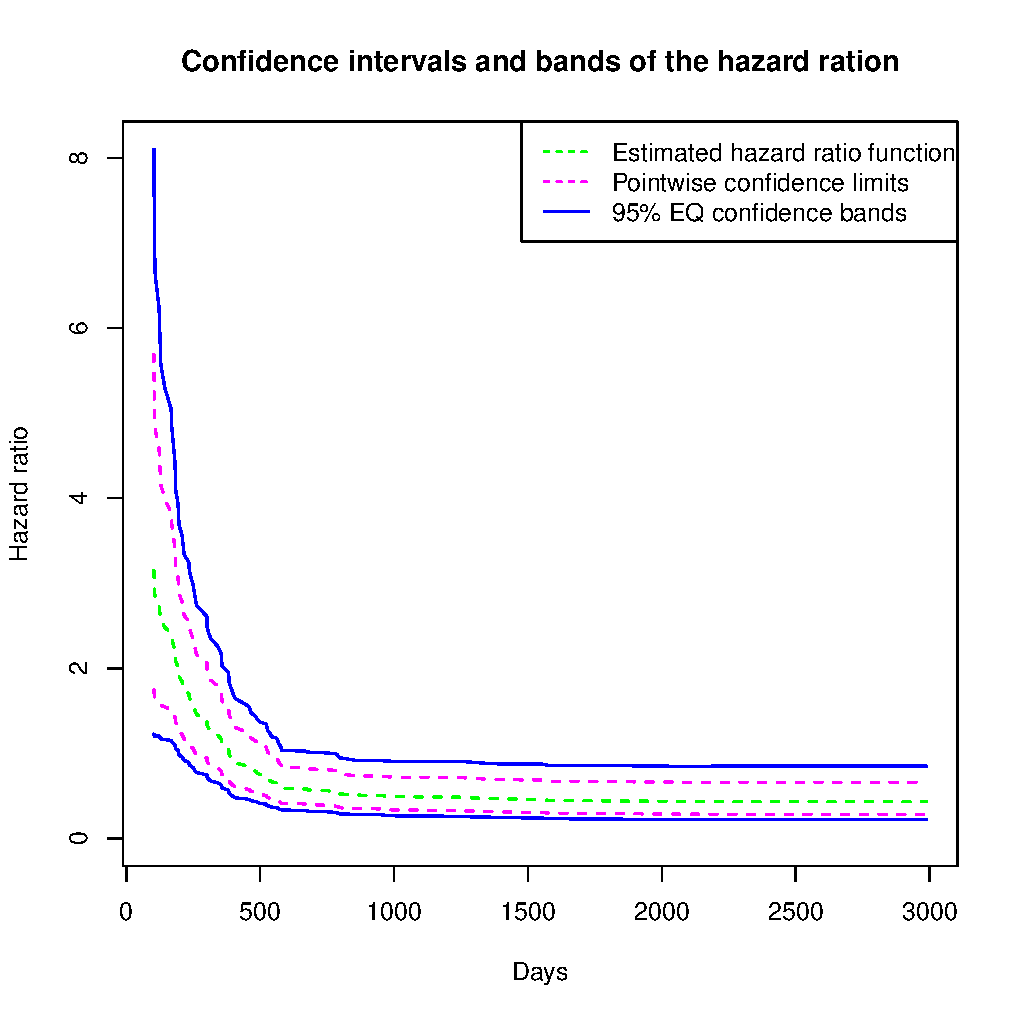
\includegraphics[width=1.0\linewidth]{plot2}}
\caption{Plotting results.}
\label{fig:plot2}
\end{figure}

\subsection{Options}\label{intervalOption}
Since the results of confidence intervals and bands depend on the estimation in section \ref{Section:estimation}, we can customize the estimates into the above functions as follows:
\insertcode{"Scripts/code14 - 2.pl"}{Performing confidence intervals and bands estimation with customized estimates.}

\section{Adaptively weighted log-rank test}\label{Section.logrank}
For testing for treatment effects with time-to-event data, the logrank test is the most popular choice and has
some optimality properties under proportional hazards alternatives.
\cite{yang2009improved} showed that
the logrank test and related tests can be improved by using
weighted logrank statistics with adaptive weights.

We can directly perform the adaptively weighted log-rank test in \cite{yang2009improved} as follows:
\insertcode{"Scripts/code18.pl"}{Performing the adaptively weighted log-rank test.}
where the dataframe $Adlgrk$ contains the results of the test, and Table \ref{Tab:IntervalBandsStructure} gives its structures.

\begin{table}[!h]
\renewcommand{\arraystretch}{1.3}
\caption{Dataframe $Adlgrk$ Structure} \label{Tab:AdlgrkStructure} \centering
\begin{tabular}{|c||c|}
  \hline
  Variables & Notes  \\
  \hline
  $pval$ & P-value from adaptively weighted logrank test. \\
  \hline
\end{tabular}
\end{table}

To get summary information about the $S3$ object obtained, we can use

\insertcode{"Scripts/code19.pl"}{}
or simply,
\insertcode{"Scripts/code19s.pl"}{Summarizing results of the adaptively weighted logrank test.}
\insertcode{"Scripts/result19.pl"}{Results of scripts.}

Because the estimation in section \ref{Section:estimation} will be used in the hypothesis test, we can customize the estimates into the above functions as follows:
\insertcode{"Scripts/code18 - 2.pl"}{Performing confidence intervals and bands estimation with customized estimates.}

\section{Two Lack-of-fit Tests}\label{Section.LacTest}
\cite{yang2012checking} proposed two omnibus tests for checking this
model, based, respectively, on the martingale residuals and the contrast between
the non-parametric and model-based estimators of the survival function.
These tests are shown to be consistent against any departure from the
model.

We use the data from section \ref{gastric.data}, and the two lack-of-fit tests can be done as follows:
\insertcode{"Scripts/code22.pl"}{Performing the two lack-of-fit tests.}
where the dataframe $LackFitTest$ contains the two lack-of-fit tests, and Table \ref{Tab:IntervalBandsStructure} gives its structures.

\begin{table}[!h]
\renewcommand{\arraystretch}{1.3}
\caption{Dataframe $LackFitTest$ Structure} \label{Tab:IntervalBandsStructure} \centering
\begin{tabular}{|c||c|}
  \hline
  Variables & Notes  \\
  \hline
  $newBest$ & Value of $\hat{\beta}$ used in the two tests.\\
  $pvalu1$ & P-value from martingale residual-based test. \\
  $pvalu2$ & P-value from contrast-based test. \\
  \hline
\end{tabular}
\end{table}

If we want to obtain the value of $LackFitTest$, it can be done with similar codes in section \ref{Section:estimation}.

\subsection{Analyzing results for Estimating confidence intervals and bands}
To get summary information about the $S3$ object, we can use

\insertcode{"Scripts/code23.pl"}{}
or simply,
\insertcode{"Scripts/code23s.pl"}{Summarizing performance of the two lack-of-fit tests.}
\insertcode{"Scripts/result23.pl"}{Results of scripts.}

Another summary function is available for plotting the survival functions. This can be done as follows:
\insertcode{"Scripts/code24.pl"}{}
or simply,
\insertcode{"Scripts/code24s.pl"}{Plotting estimates' process of the two lack-of-fit tests.}

\begin{figure}[H]
\center{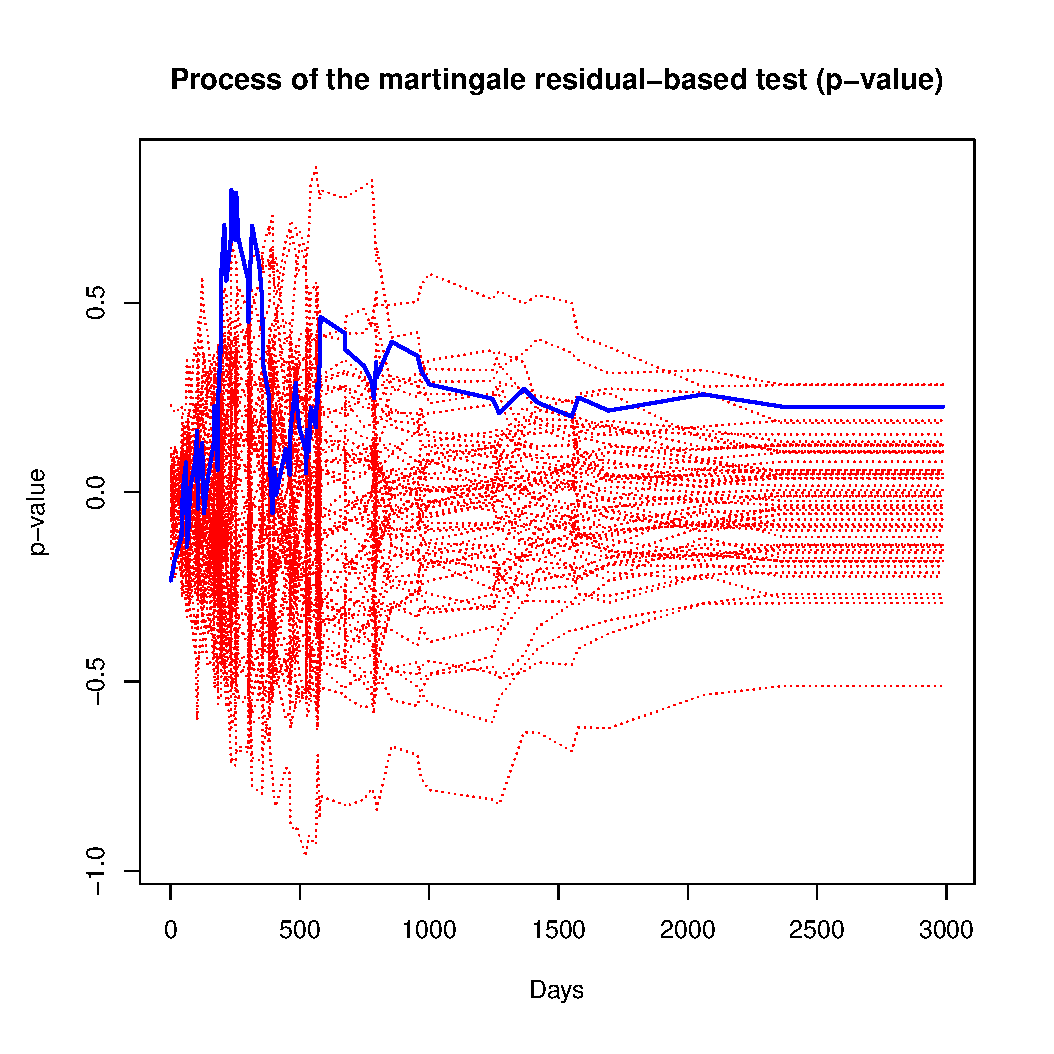
\includegraphics[width=0.8\linewidth]{plot3}}
\caption{Plotting results.}
\label{fig:plot3}
\end{figure}
\begin{figure}[H]
\center{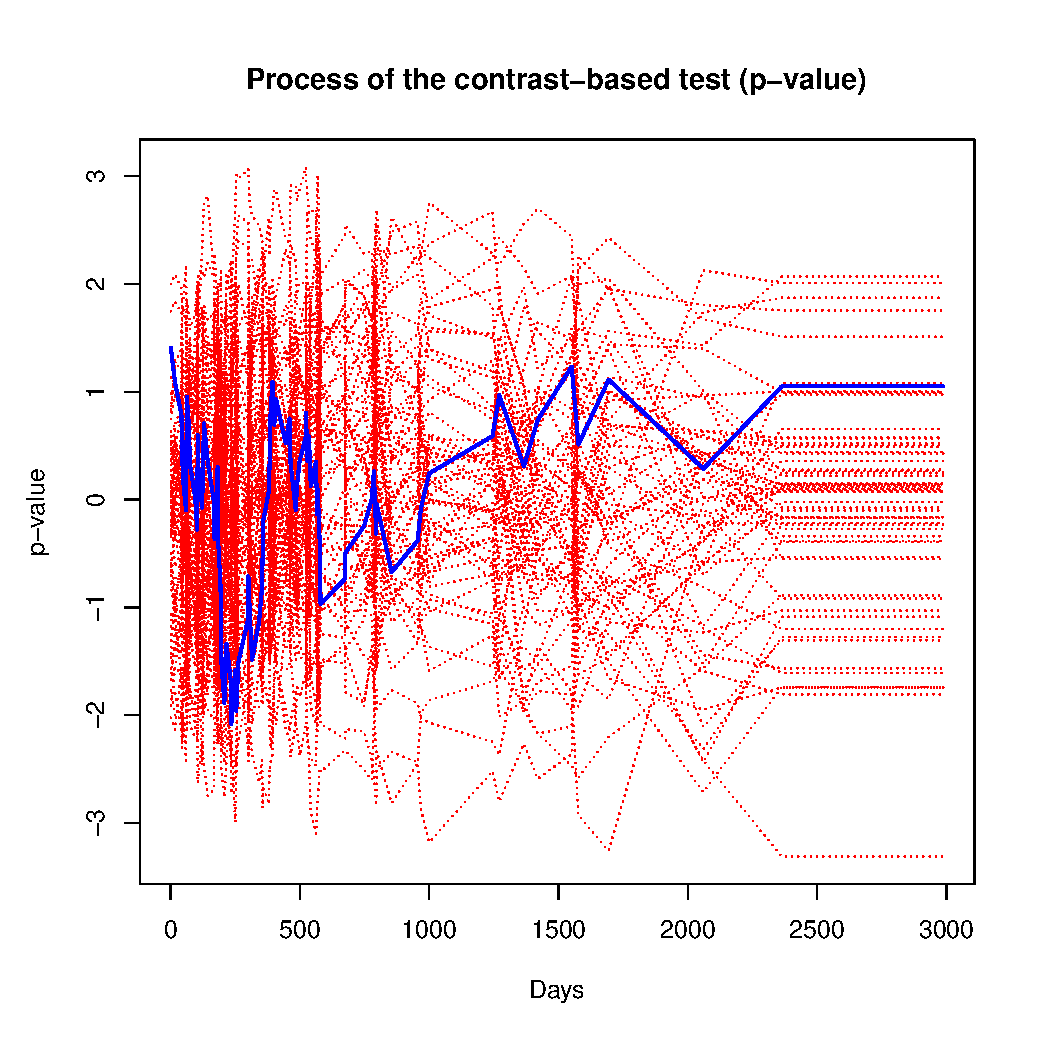
\includegraphics[width=0.8\linewidth]{plot4}}
\caption{Plotting results.}
\label{fig:plot4}
\end{figure}

\subsection{Options}
The parameter $repNum$ sets number of random variables to be used the two lack-of-fit tests, and its default value is $1000$. Assume we would like to use only $100$ random variables instead. This can be done as follows:
\insertcode{"Scripts/code20.pl"}{Loading YPmodel package and performing estimating process.}

\section{All-in-one Function}\label{Section.All}

In the section \ref{Section.Model} - \ref{Section.LacTest}, we see how different functions can be called to analysis survival data with the model of Yang and Prentice (YPmodel) (using data in section \ref{gastric.data}). The whole process (with default parameters) can be summarized with
\insertcode{"Scripts/code25.pl"}{Summary of functions.}

To simplify those procedures, we also provide one all-in-one function for YPmodel.
\insertcode{"Scripts/code26.pl"}{All-in-one Function.}
where the parameters can be customized as follows:
\insertcode{"Scripts/code26 - 2.pl"}{All-in-one Function with customized parameters.}

And the S3 function "plot" and "summary" can be used to demonstrate the all four above results
\insertcode{"Scripts/code26 - 1.pl"}{Demonstrating the overall results.}

\begin{remark}
We can directly load the text file when using function "YPmodel" as follows:
\insertcode{"Scripts/code27.pl"}{Performing YPmodel with text files.}
\end{remark}

\section{Conclusions}\label{Section.Conclusions}
We have implemented the methodology described above in an R package, called YPmodel.
This would be used by analysts and others whose task is to analysis of the
comparison of failure times between a treated and control group under inde-
pendent censorship.

To estimate survival data using YPmodel, the user will usually follow three
basic steps in the following order:
\begin{enumerate}
  \item Preparing data set in section \ref{Section.Model}.
  \item Estimate the model parameters in section \ref{Section:estimation}.
  \item Estimate confidence intervals and bands for the hazard ratio function in section \ref{Section.Intervals}.
  \item Perform the Adaptively weighted log-rank test in section \ref{Section.logrank}.
  \item Perform the lack-of-fit tests in section \ref{Section.LacTest}.
\end{enumerate}
and section \ref{Section.All} provides an all-in-one method to use step $2$ - $5$. Plus, each step can be independently performed.
Use "help(function)" for more
specifics about each function described below and details about its arguments.

\section{Appendix}

There are several parameters used by the package.
The correspondence of these parameters to their argument names and default values used
in YPmodel version $1.0$ is shown in Table \ref{Tab:Appendix}.

\begin{table}[!h]
\renewcommand{\arraystretch}{1.3}
\caption{Dataframe $Adlgrk$ Structure} \label{Tab:Appendix} \centering
\begin{tabular}{|c||c|c|}
  \hline
  Parameters & Default values & Notes  \\
  \hline
  $startPoint$ & $c(0,0)$ & Define the start point of the iteration for $\hat{\beta}$. \\
  $nm$ & $\log(100)$ & Define a bound for $\hat{\beta}$. \\
  $maxIter1$ & $50$ & Define out-cycle iteration numbers. \\
  $maxIter2$ & $20$ & Define inner-cycle iteration numbers. \\
  $repNum$ & $1000$ & Number of iterations in the two lack-of-fit tests. \\
  \hline
\end{tabular}
\end{table}

%----------------------------------------------------------------------------------------
%	BIBLIOGRAPHY
%----------------------------------------------------------------------------------------

\bibliographystyle{plainnat}
\bibliography{YPmodel}

%----------------------------------------------------------------------------------------

\end{document}
